\documentclass[10pt]{article}
\usepackage[utf8]{inputenc}

\usepackage{geometry}
\usepackage{graphicx}

\geometry{portrait, margin=1.5in}

\begin{document}
\section{Exercise 1 - Your wish is my command, Reloaded }
\subsection{Local co-op Multiplayer Functional Requirements}

A list of functional requirements considered for the implementation of local co-op multiplayer using the MoSCoW method described in the previous section.

\subsubsection{Must Haves}
The local co-op multiplayer must meet the following requirements:
\begin{itemize}
	\item A multiplayer game shall contain two spaceships.
	\item The game shall be able to load a multiplayer game.
	\item The first spaceship shall be controlled using predefined keys on the keyboard.
	\item The second spaceship shall be controlled using predefined keys on the keyboard.
\end{itemize}

\subsubsection{Should Haves}
The local co-op multiplayer should meet the following requirements:
\begin{itemize}
	\item The User Interface shall have a menu to select between single or multiplayer games.
	\item The User Interface shall display two different score elements and life elements for different players.
	\item Each spaceship shall have an equal initial movement speed.
	\item Powerups work for individual spaceships.
\end{itemize}

\subsubsection{Could Haves}
The local co-op multiplayer could meet the following requirements:
\begin{itemize}
	\item The game shall end after one of both players runs out of lives.
	\item The game shall display the winner after the game ends.
	\item The player wins if he/she has the highest score.
	\item The game shall spawn a powerup with the ability to freeze the other player for a predefined amount of time.
\end{itemize}

\subsubsection{Would/Won't Haves}
The local co-op multiplayer won't meet the following requirements:
\begin{itemize}
	\item Spaceships shall collide.
\end{itemize}
\newpage

\subsection{Class responsibilities and collaborations}


The following new classes were created for the implementation of the new local multiplayer feature.
In the table the responsibilities and collaborations are presented for every class.
\begin{center}
    \begin{tabular}{ | p{4.5cm} | p{3cm} | p{3cm} | p{3cm} | p{1cm} |}
  \hline
    Class & Responsibility & Collaborates with & Super & Sub \\ \hline
   MultiPlayerGame & Players  & & Game & \\ \hline
   GameUIController & drawing the UI elements & MultiPlayerGame  & GameUIController  & \\ \hline
 MultiPlayerGameUIController & Key control & MultiPlayerGame  & GameUIController  & \\ \hline
 SinglePlayerGameUIController & Key control & Game  & GameUIController  & \\ \hline
   MenuUIController& Conrol menu & MultiPlayerGameUI- Controller  &   &  \\ \hline
   UiElementMultiSpaceShips& draw multiple spaceShips & MultiPlayerGameUI- Controller  &  &  \\ \hline
 MultiGameScore & score display multiple players &  MultiPlayerGame  &  Score  & \\ \hline
 MultiGameLives &  lives display multiple players & MultiPlayerGame  & Lives  & \\ \hline
 MultiSpaceShipsController& Control multiple spaceships & SpaceShip  & SpaceShipController &  \\ \hline
 MultiPlayerPowerUpController& Control powerups for multiple players & MultiPlayerGame   & PowerUpController &  \\ \hline

    \end{tabular}
\end{center}

Furthermore we have to replace the check if the alien is at the same height as a spaceship from AlienController to the SpaceshipController. \newline
And replace the score add call to the multiplayercollisions.
\newpage
\subsection{Multiplayer UML}
The UML is as following:
\begin{figure}[ht!]
	\centering
	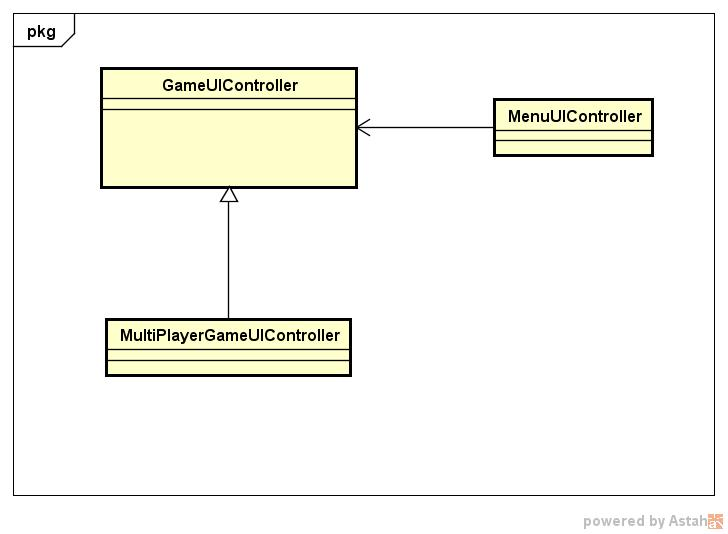
\includegraphics[width=10cm]{GameUI.jpg}
	\caption{MultiGame UI UML}
	\label{fig:1-1MultiGameUI}
\end{figure}
\begin{figure}[ht!]
	\centering
	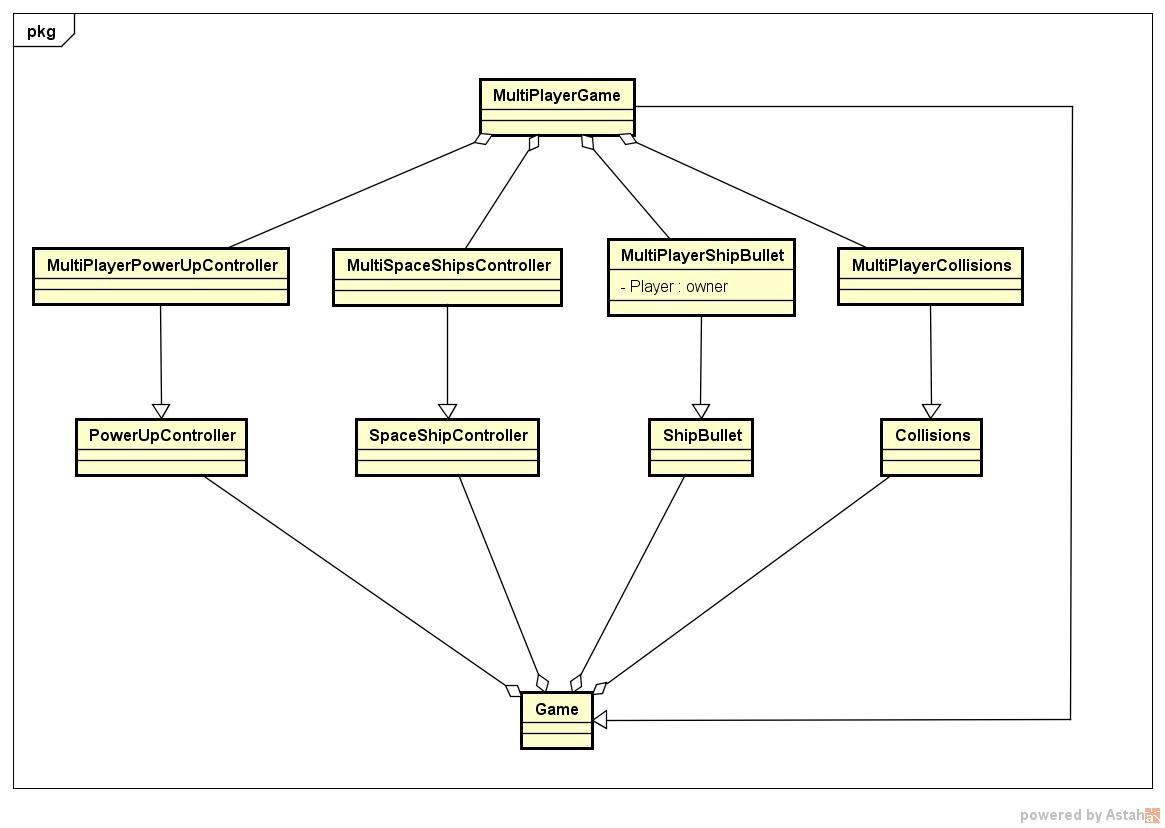
\includegraphics[width=15cm]{MultiGame.jpg}
	\caption{MultiGame UML}
	\label{fig:1-1MultiGameGame}
\end{figure}

\end{document}
